\documentclass[conference,10pt]{IEEEtran}
% Build: ./build.sh  (figures: make_figures.py; LaTeX: pdflatex x2)
\usepackage[T1]{fontenc}
\usepackage{amsmath,amssymb}
\usepackage{graphicx}
\usepackage{booktabs}
\usepackage{multirow}
\usepackage{xcolor}
\usepackage{tikz}
\usetikzlibrary{positioning,arrows.meta,fit}
\usepackage{microtype}
\usepackage[hidelinks]{hyperref}
\usepackage{url}

\newcommand{\todo}[1]{\textcolor{red}{\textbf{[TODO: #1]}}}
\newcommand{\file}[1]{\texttt{\small #1}}
\newcommand{\dJ}{\Delta J}

\begin{document}

\title{Validated Ensembles, Physics-Gated Post-Processing and Selection-Faithful Queue Forecasting for TrafficFlowBench\\
{\large Team Hack2Publish (Kaggle: \texttt{hosen42})}}

\author{\IEEEauthorblockN{Md. Hamid Hosen\IEEEauthorrefmark{1},
Md. Foysal Emon Shanto\IEEEauthorrefmark{2} and
Md. Esfer Abdus Sami\IEEEauthorrefmark{3}}
\IEEEauthorblockA{\IEEEauthorrefmark{1}Dept. of Computer Science and Engineering, East Delta University, Chattogram, Bangladesh}
\IEEEauthorblockA{\IEEEauthorrefmark{2}Dept. of Computer Science and Engineering, Jashore University of Science and Technology, Jashore, Bangladesh}
\IEEEauthorblockA{\IEEEauthorrefmark{3}Dept. of Computer Science and Engineering, North South University, Dhaka, Bangladesh\\
Email: mdhamidhosen4@gmail.com, foyshalsk348@gmail.com, esfer.sami.me@gmail.com}}

\maketitle

\begin{abstract}
We describe our solution to the 2026 IEEE Big Data Cup \emph{TrafficFlowBench}, a four-task freeway benchmark
(state reconstruction, queue forecasting, physical consistency and origin--destination estimation) scored as one
weighted total. Our final submissions reach a public-leaderboard score of 0.88281, up from 0.80939 for the
public notebook we started from. The Task~1 reconstruction is a residual ensemble of 17 gradient-boosted members
(LightGBM, CatBoost, XGBoost) trained on the training months plus \emph{transductive} rows from the released
cells of the target months. A dedicated specialist handles the 90-minute blackouts after Task~2 forecast origins, and a
low-rank tensor completion of the month's own flow field adds a further member. Task~3 is improved only through Task~1:
an FD-gated reconciliation and a 1-D total-variation smoother move the reconstructed density towards the
fundamental diagram and remove noise that breaks conservation. For Task~2 we found that the official windows are
selected with a persistence cap evaluated on the \emph{full} state. Training the ongoing-queue model on windows
selected the same way gave our largest single gain after the first model. Onset queues are forecast at $T{+}30$ only,
with a CatBoost classifier and an expected-IoU decoder. Task~4 uses the organizer's prior-regularised NNLS. All
changes passed through day-blocked cross-validation, a pseudo-March evaluation and pre-registered gates. Every
Task~2 forecast uses only data stamped at or before its origin $T$. We report the full progression, the
offline-to-leaderboard transfer and a list of negative results.
\end{abstract}

\section{Introduction}
TrafficFlowBench~\cite{tfb} asks four questions about ten synthetic but calibrated directional freeway corridors
(``panels'') at 5-minute resolution: fill in masked detector cells (Task~1), forecast which links are queued in
the next 30 minutes (Task~2), be physically consistent while doing Task~1 (Task~3), and recover path flows from link
counts (Task~4). The score is
\begin{equation}
\begin{split}
S = {}&0.35\,S_\text{state} + 0.30\,S_\text{queue}\\
&+ 0.05\,S_\text{FD} + 0.10\,S_\text{LWR} + 0.20\,S_\text{ODME},
\end{split}
\label{eq:score}
\end{equation}
where $S_\text{physics}=S_\text{FD}/3+2S_\text{LWR}/3$ carries weight 0.15. The public leaderboard (LB) scores the
validation month (March 2031); the private LB scores April 2031. The training split has 273 days with released
answers.

\textbf{Contributions.}
(i) A transductive residual ensemble for Task~1 that also improves Task~3, with an explicit blackout specialist and a
month-level low-rank member (Sec.~\ref{sec:t1}).
(ii) Two physics-based post-processing steps for Task~3 that can be applied to any reconstruction (Sec.~\ref{sec:t3}).
(iii) A reconstruction of the official Task~2 window selector, and selection-faithful training that follows from it
(Sec.~\ref{sec:t2}).
(iv) A validation protocol of day-blocked folds, pseudo-March windows and pre-registered gates. It recorded how
offline gains transfer to the LB and helped us avoid tuning to LB noise (Sec.~\ref{sec:val}).
(v) A documented list of what did not work (Sec.~\ref{sec:neg}). Fig.~\ref{fig:pipeline} summarises the final pipeline.

Organizer requirements for this report (forum post 744187) are a PDF ``describing your method, your analysis and
your results across the four tasks''. There is no template and no page limit. Every number below is traceable to a file in
our repository. Files are named in \file{typewriter}, and the main log is \file{experiments/TRACKER.md}. Numbers
that are estimates are marked as such.


\begin{figure}[t]
\centering
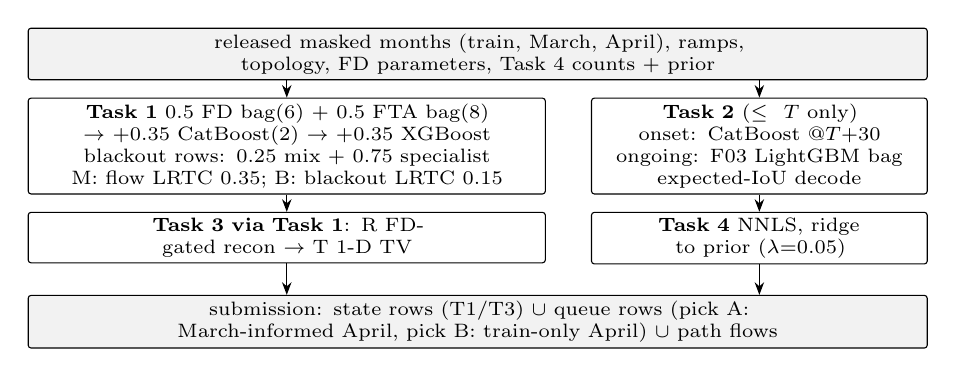
\begin{tikzpicture}[font=\scriptsize, node distance=2.2mm,
  box/.style={draw, rounded corners=1pt, align=center, inner sep=2pt, minimum height=5mm},
  arr/.style={-{Stealth[length=1.6mm]}, thin}]
\node[box, fill=gray!10, text width=0.93\columnwidth] (rel) {released masked months (train, March, April), ramps, topology, FD parameters, Task~4 counts + prior};
\node[box, below=of rel.south west, anchor=north west, text width=0.53\columnwidth] (t1) {\textbf{Task 1} 0.5 FD bag(6) + 0.5 FTA bag(8)\\ $\to$ +0.35 CatBoost(2) $\to$ +0.35 XGBoost\\ blackout rows: 0.25 mix + 0.75 specialist\\ M: flow LRTC 0.35; B: blackout LRTC 0.15};
\node[box, below=of t1, text width=0.53\columnwidth] (t3) {\textbf{Task 3 via Task 1}: R FD-gated recon $\to$ T 1-D TV};
\node[box, below=of rel.south east, anchor=north east, text width=0.34\columnwidth] (t2) {\textbf{Task 2} ($\le T$ only)\\ onset: CatBoost @$T{+}30$\\ ongoing: F03 LightGBM bag\\ expected-IoU decode};
\node[box, below=of t2, text width=0.34\columnwidth] (t4) {\textbf{Task 4} NNLS, ridge to prior ($\lambda{=}0.05$)};
\node[box, fill=gray!10, below=4mm of t3.south west, anchor=north west, text width=0.93\columnwidth] (sub) {submission: state rows (T1/T3) $\cup$ queue rows (pick A: March-informed April, pick B: train-only April) $\cup$ path flows};
\draw[arr] (rel.south -| t1.north) -- (t1.north);
\draw[arr] (t1) -- (t3);
\draw[arr] (rel.south -| t2.north) -- (t2.north);
\draw[arr] (t2) -- (t4);
\draw[arr] (t3.south) -- (t3.south |- sub.north);
\draw[arr] (t4.south) -- (t4.south |- sub.north);
\end{tikzpicture}
\caption{Final pipeline. The two picks share every state, March queue and path-flow row; they differ only in 200 April queue rows.}
\label{fig:pipeline}
\end{figure}

\section{Problem, data and rules}\label{sec:problem}
\textbf{Task 1 (state).} Every calendar day is masked in one regime (R1/R2/R3 = 20/30/50\,\% of eligible cells).
The submission gives speed and flow for every target cell. $S_\text{state}=0.54\max(0,1-\text{RMSE}_v/25)
+0.46\max(0,1-\text{RMSE}_{q/\text{lane}}/600)$, averaged over regimes, then panels.
\textbf{Task 2 (queue).} Each of 8 panels has 5 \emph{onset} and 5 \emph{ongoing} windows per split. Each window gives 60 minutes of
history before an origin $T$, and the released row at $T$ may also be used. The target is a binary queue map (speed $\le
0.6\,v_f$ of the noise-free state) over $T{+}5,\dots,T{+}30$ for every link. The score is a per-window space-time IoU, averaged
window $\to$ condition $\to$ panel.
\textbf{Task 3 (physics)} is computed from the Task~1 file. $S_\text{FD}$ measures the distance to the
fundamental diagram (FD). $S_\text{LWR}$ measures violations of LWR vehicle conservation~\cite{lwr1}, $N(t{+}1)-N(t)=\Delta t(q_\text{in}+r_\text{on}-q_\text{out}-r_\text{off})$, with
$N=(q/\max(v,1))L$. It uses organizer-held boundary fluxes, so it cannot be scored locally.
\textbf{Task 4 (ODME)} asks for path flows given the incidence matrix $A$, link counts $c$ and a weak prior $b$.

\textbf{Time-stamp rule.} Task~1 is offline, so any released observation of the split may be used (organizer, post 742068).
For Task~2, a forecast with origin $T$ may use released data stamped $\le T$. That covers the training split, earlier
days of the same split and, for April, all of March (posts 742068, 745700, 748789). It may not use ramp values inside
the horizon or later mainline observations. At award review the organizers rerun Task~2 with every row after each
window's $T$ removed, and the predictions must not change (post 749601). We read that post strictly:
every model, threshold and selection choice that affects April rows was made on training and March evidence only.

\section{Validation methodology}\label{sec:val}
\subsection{Folds and replicas}
All Kaggle runs share frozen folds: 3 contiguous day blocks for Task~1 and 4 for Task~2. Task~1 candidates are also scored on a
\emph{validation-month internal holdout}. In it, 15\,\% of the released March cells (seed 7) are hidden in every view and never used as
a target. This holdout followed the LB closely early on: for example, the low-rank features gave a predicted $+0.0013$ and an observed
$+0.0015$ (\file{TRACKER}, EXP\_017).

For Task~2 we wrote a replica of the official selector. The history is $[T{-}60,T)$ with $\ge70\,\%$ eligible cells. A window is
\emph{ongoing} if some link has $\ge2$ queued observations, otherwise \emph{onset}. The horizon must contain a queue,
the persistence IoU must be $\le0.9$, and picks are greedy with 360-minute spacing. The replica reproduces 39/40 official onset origins
on the training split. The first version reproduced only 14/40 \emph{ongoing} origins. Evaluating the persistence cap on a time-filled
state instead (linear interpolation along time over gaps up to 36 slots, applied to all cells) reproduces 36/40, and 39/40 within
5 minutes (\file{analysis/t2lab/README.md}). This filled state is used only to select windows, never as a feature.

\subsection{Pseudo-windows and pseudo-March}
The replica produces \emph{pseudo-windows} on the training split: about 2{,}000--3{,}000 ``official-like'' ongoing windows (greedy
restarted every day) and the run-start windows. Models are scored out of fold with the official IoU aggregation and paired
bootstraps by window within panel. Since March and April come from a new scenario (re-drawn ramp demand and a different set of
active bottlenecks; \file{analysis/CAPACITY\_SCENARIO\_2026-10-11.md}), we also built \emph{pseudo-March} windows from the released
masked March layer. Their labels are observed cells only, and they are a decision aid for scenario-dependent choices. A
``many-day'' variant uses March days $<15$ for fitting and days $\ge15$ for evaluation. It mimics April, which can use all
of March.

\subsection{The Task~1 J proxy and pre-registered gates}
From October on, every Task~1/3 candidate was evaluated in a paired lab on 4 panels $\times$ 2 masked months (16
fold views). Released cells are hidden in the official run pattern, and blackouts are simulated where official Task~2 windows
would put them. The metric is the score-weighted proxy
\begin{equation}
J = 0.35\,S_\text{state} + 0.10\,\widetilde S_\text{LWR} + 0.05\,S_\text{FD},
\end{equation}
where $\widetilde S_\text{LWR}=1-\sum|\Delta N_\text{pred}-\Delta N_\text{obs}|/\sum|\Delta N_\text{obs}|$ uses released
truth outside the target cells. On D12\_I405\_S the naive baseline gives a proxy $S_\text{physics}\approx0.39$, against the official 0.355
(\file{TRACKER}, validation design). Before any result was computed, each round wrote a gate into
\file{analysis/t1lab/t1div\_lib.py}, with the time recorded. For a new member the gate is: $\dJ\ge+0.0003$ after the
full post-processing, a 95\,\% bootstrap CI lower bound $>0$, $\ge7/8$ panel-months positive, and a margin of $\ge+0.00015$ over a
control that simply adds another LightGBM seed at the same weight. Post-processing and weight changes used
$\dJ\ge+0.0002$. Results that were not gate-eligible (post-hoc) are labelled as such below.

\subsection{Footprint-matched pseudo-March (FM-PM)}
Plain train-OOF and pseudo-March deltas mispredicted the LB effect of ongoing changes (MAE 0.0013--0.0015 in $S$). The FM-PM
estimate is label-free on the target month. It decodes both candidate files, finds the official windows whose decision changes,
and prices each with the paired pseudo-March delta of lab windows from the same panel, a similar time of day ($\pm2$\,h) and a similar change
size. The mean is then scaled by the weight of one window. On the five ongoing LB probes it was evaluated on, FM-PM on the
\emph{validation} footprint had MAE 0.0005 (\file{TRACKER} EXP\_T2\_XFER; Fig.~\ref{fig:transfer}, right). FM-PM was
calibrated after these probes, so this MAE is in-sample. Following the strict time-stamp reading above, we never used FM-PM
computed on April windows as a binding criterion for April rows.

\subsection{Leaderboard noise and the keep rule}
With 40 windows per condition, one ongoing probe has an LB standard deviation of $\pm0.0012$--$0.0027$ and one onset probe
$\pm0.003$--$0.005$ (\file{TRACKER} EXP\_T2\_XFER). A public delta below $+0.0001$ was never accepted as a gain (e.g.\ F1 $+0.00002$, J1
$+0.00003$). Most Task~1 increments in our final phase were kept because a gate had passed offline, not because of their LB delta.

\section{Task 1: state reconstruction}\label{sec:t1}
\subsection{Residual members with transductive rows}
Every member predicts \emph{residuals} of speed$/v_f$ and flow per lane with respect to a per-station linear interpolation in time.
Features include the interpolation itself, neighbour stations at the same instant, a per-day rank-3/rank-5 SVD reconstruction of the
interpolated fields, occupancy, characteristic-kernel (``ASM'') averages along $\pm80$ and $\pm18$\,km/h waves, and, in the newer
``FD'' family, 20 columns of FD-implied densities and flows of several speed views. Profile features were dropped because the
profile-free model was better on 10/10 panels. Training rows come from the training split with simulated 90-minute gaps. They are
augmented with \emph{transductive} rows: in 2--4 rounds, 20\,\% of the released cells of the validation and private months are hidden
and used as targets. This is legal because Task~1 is offline (post 742068). It added $+0.0020$ on the holdout (10/10 panels) and
$+0.0017$ on the LB (\file{TRACKER} EXP\_T1\_trans).

\begin{table}[t]
\centering
\caption{Task 1 progression on the validation-month internal holdout (composite $S_\text{state}$; \file{TRACKER}).}
\label{tab:t1hold}
\begin{tabular}{lcc}
\toprule
Model & Holdout & Public LB \\
\midrule
Temporal-interpolation base (re-implemented) & 0.9141 & -- \\
LightGBM residual, profile-free & 0.9307 & 0.84855 \\
+ per-day rank-3 SVD features & 0.9343 & +0.0015 \\
+ rank-5 / occupancy / cross-day low rank & 0.9350 & -- \\
255 leaves, 900 trees, $2\times$ rows & 0.9374 & -- \\
511 leaves, 1500 trees, $4\times$ rows & 0.9386 & +0.0011 \\
+ transductive rows (FT) & 0.9406 & +0.0017 \\
+ ASM wave features (FTA) & +0.0005 & +0.0003 \\
\bottomrule
\end{tabular}
\end{table}

\subsection{The final ensemble}
The final Task~1 file of both picks is produced as follows (constants in \file{consolidation/tfb/config.py}, kernel docstrings in
\file{submissions/76\_K9/tfb-k9.py}):
\begin{enumerate}
\item $m_0 = 0.5\,\overline{\text{FD}} + 0.5\,\overline{\text{FTA}}$, where FTA is a bag of 8 LightGBM members (seeds 0--7, 2--4
transductive rounds) and FD is a bag of 6 (three FD-feature seeds, a simulated-blackout member and two members with 9 ramp features).
All are LightGBM~\cite{lgbm} with 511 leaves, learning rate 0.04 and 1500 trees.
\item $m_1 = 0.65\,m_0 + 0.35\,\overline{\text{CatBoost}}$~\cite{catboost}: two seeds, each the mean of a depth-8 and a depth-10 model, on the 94 FD columns.
\item $m_2 = 0.65\,m_1 + 0.35\,\text{XGBoost}$~\cite{xgb} (hist, depth 9, 1500 rounds).
\item \textbf{Blackout override.} About 1.9\,\% of the target rows lie in $(T, T{+}90\,\text{min}]$ of an official Task~2 window, where the whole
mainline is dark. These rows get $0.25\,m_2 + 0.75\,$BSPEC. The specialist BSPEC is trained on simulated blackouts placed exactly as
the official selector places them (onset queue first at $T{+}30$, ongoing run-starts). It has 30 timing columns and ramp flows over the gap,
which are released at the normal rate inside mainline blackouts (\file{TRACKER} DIAG\_RAMP).
\item \textbf{Step M.} On ordinary rows, $q\leftarrow\max(0.65q+0.35\,q_\text{LRTC},20)$. Here $q_\text{LRTC}$ is an EM low-rank tensor
completion of the month's own released flow cube (days $\times$ 288 slots $\times$ stations, each station normalised by its mean,
60 iterations, mean of the truncated-SVD projections of the 3 unfoldings, ranks $(24,40,10)$), in the spirit of
HaLRTC~\cite{liu2013}.
\item \textbf{Step B.} On blackout rows, $v\leftarrow\text{clip}(0.85v+0.15v_\text{LRTC},3,1.05v_f)$ and $q\leftarrow\max(0.85q+0.15q_\text{LRTC},20)$,
with speed ranks $(8,20,20)$ and flow ranks $(8,40,10)$.
\item Steps R and T of Sec.~\ref{sec:t3}.
\end{enumerate}
The CatBoost, XGBoost and LRTC members were each added after passing the pre-registered gate:
$\dJ=+0.00071$, $+0.00056$ and $+0.00054$ (all 8/8, Table~\ref{tab:gates}). The blackout specialist reduced blackout-cell speed RMSE by 6\,\% relative to
the previous ramp member ($\dJ=+0.00044$, 8/8). The ranks of step M and the step B blend come from a \emph{post-hoc} lead of round 5,
$\dJ=+0.00037$ [+0.00030, +0.00045], 8/8. We shipped it as K9 with an expected LB gain of about $+0.0002$ (observed $+0.00022$).

\begin{table}[t]
\centering
\caption{Pre-registered Task 1 gate rounds (\file{analysis/t1lab/t1div\_lib.py}); $\dJ$ after recon + TV, 8 panel-months.}
\label{tab:gates}
\footnotesize\setlength{\tabcolsep}{3pt}
\begin{tabular}{@{}llrcl@{}}
\toprule
Rd & Candidate & $\dJ$ ($10^{-4}$) & +/8 & Verdict \\
\midrule
1 & CatBoost FD member @0.35 & 7.1 & 8 & PASS \\
1 & day-grid U-Net @0.15 & 0.6 & 6 & FAIL \\
2 & XGBoost FD member @0.35 & 5.6 & 8 & PASS \\
2 & CatBoost on old FTA columns & 0.8 & 6 & FAIL \\
3 & XGB seed 2, ExtraTrees, ridge, log-target & $\le$0.2 & $\le$4 & FAIL \\
3 & re-weight XGB to 0.6 & 1.7 & 7 & FAIL \\
4 & flow-only LRTC member @0.35 & 5.4 & 8 & PASS \\
4 & density interp.\ post-proc.\ (27 cfg) & $-4.1$ & 0 & FAIL \\
4 & neighbour smoothing + FD cap & 0.6 & 6 & FAIL \\
5 & LRTC rank mean / NNLS stack & 1.8 / 2.1 & 8 & FAIL \\
5 & LRTC on blackout rows (blkVQ@0.15) & 1.85 & 7 & FAIL \\
5$^*$ & ranks (24,40,10) + blkVQ@0.15 & 3.7 & 8 & post-hoc \\
7 & kNN-day analog member & 0.5 & 6 & FAIL \\
7 & 3-rank LRTC ensemble & 0.4 & 6 & FAIL \\
\bottomrule
\end{tabular}
\end{table}

\section{Task 3: physics through Task 1}\label{sec:t3}
Task~3 cannot be submitted separately, and its LWR term is computed against organizer-held boundary fluxes.
A local sensitivity study on D12\_I405\_S (60 days) showed how sensitive the proxy is to noise. Temporal interpolation scores 0.52, while truth plus only 1\,km/h of
speed noise or 1\,\% of flow noise falls to about 0.89. $S_\text{LWR}$ is therefore set mainly by the per-cell noise of the
reconstructed density, not by the flux balance itself. The station-to-station conservation estimate is 10--28 times the LWR
signal (\file{TRACKER} EXP\_T1\_LWRPROJ). We therefore improve the reconstructed density directly:

\textbf{Step R: FD-gated reconciliation.} At target rows with $v<0.6\,v_f$ the per-lane density $k=q/(\text{lanes}\cdot v)$ is moved
towards the congested FD branch implied by the predicted speed, $k_\text{FD}(v)=w\,k_j/(v+w)$ with $w=\text{cap}/(k_j-k_c)$.
The FD parameters are averaged per link exactly as the organizer scorer does. With $r=\text{clip}(k_\text{FD}/k,e^{-0.5},e^{0.5})$, we set
$v'=\text{clip}(v\,r^{-0.75},3,1.05v_f)$ and $q'=\max(q\,r^{0.25},20)$, so 75\,\% of the correction goes to speed. Links with implausible FD
parameters ($w\notin[8,40]$\,km/h or $k_j/\text{lane}\notin[60,200]$; 10 links) are excluded. A panel would also be excluded if the
released congested cells disagreed with its FD (median $>2\,\%$ or IQR outside $\pm5\,\%$); no panel was. The step
changes 4\,\% of state rows and gave LB $+0.00167$, the largest Task~3 gain.

\textbf{Step T: 1-D total variation.} Inside every maximal temporal run of target cells per station, the per-lane density is
smoothed by a TV-L2 denoiser (300 Chambolle dual iterations~\cite{chambolle2004}), anchored to the released cells
just before and after the run. The strength depends on the run's mean density (free cells $\tau=0.0075$, gated cells $0.02$). In gated cells the
density change goes 75\,\% to speed, and in free cells all of it goes to flow. LB $+0.00026$. A scan of 294 recon/TV variants found nothing
better than $+0.0002$ in proxy $J$, so both steps were frozen.

The Task~1 members also help Task~3. The flow LRTC member gains mostly through $\widetilde S_\text{LWR}$ ($+0.0043$ against $+0.00034$ in
$S_\text{state}$; \file{TRACKER} EXP\_T1\_DIV4), because averaging with an estimator of a different kind removes
part of the per-cell noise.

\section{Task 2: queue forecasting}\label{sec:t2}
\subsection{Cell classifier and decoder}
Each window is turned into one row per (link, horizon step). Features are computed only from the 60-minute history, the
released row at $T$, static link attributes and priors: speed ratios and their trends, queue run lengths, neighbour and distance-to-queue
features, released ramp flows at $T{-}3..T{-}1$ (ongoing only), occupancy, and train-split location/time priors
$P(\text{queued}\mid\text{link},\text{slot}\pm2,\text{weekday class})$. A lab perturbation test checked the timing: changing any data after $T$,
before $T{-}60$, or ramp flows at $\ge T$ leaves every feature unchanged (\file{analysis/t2lab/README.md}). Probabilities are decoded per
window by an \emph{expected-IoU} rule. Cells are sorted by $p$, and the top-$m$ are chosen to maximise
$\sum_{i\le m}p_i/(m+\sum_{i>m}p_i)$. This decoder beat fixed thresholds, morphology and per-step decoding (\file{TRACKER} EXP\_T2\_D).

\subsection{Onset}
Post 742350 (organizer) and our own counts on the training windows (39/40 official, 96.9\,\% of pseudo-windows) show that every
onset queue first appears at $T{+}30$. So onset is a one-step problem: \emph{which links} queue at $T{+}30$. A CatBoost classifier
(depth 8, 600 iterations, seed 0) on the step-6 rows replaced the LightGBM blend (LB $+0.0006$). For March rows (``sp4'') the three
prior columns are blended per cell with a \emph{same-scenario} prior estimated from released March days strictly before the window's
day, $a=n/(n+4)$ with $n$ visible days (LB $+0.00104$, the only onset change besides CatBoost that transferred).

\subsection{Ongoing: selection-faithful training}
Training on the replica's original ``current-style'' pseudo-windows (Sec.~\ref{sec:val}) mostly produced stable queues that the official
selector never picks, because its persistence cap rejects them. Training instead on selection-faithful windows (all faithful candidates
on a 15-minute grid with weight 0.3, plus faithful run-starts with weight 1.0; ``F03'') improved official-like OOF IoU from 0.8387 to
0.8751/0.8806 (4/4 folds) and pseudo-March by $+0.021$ (6/8 panels). On the LB it gave $+0.0047$, the largest gain after the first model.
The March ongoing model (``fs4occ'') is a bag of 4 LightGBM models (511 leaves, 1800 trees): two prior-free and two
``identity'' column sets with 2 seeds each. They use \emph{all finite} released values as inputs, including ineligible-but-valued
cells (about 7\,\%; LB $+0.0009$), plus 13 occupancy features ($+0.0001$).

\subsection{April rows and the two final picks}
Train-split evidence and March evidence disagree on one question: does April share March's scenario? The release
configuration says validation and private use one scenario seed, while the data README says the two months were ``generated
independently''. On many-day pseudo-March, models fitted on train plus released-March windows clearly beat train-only models (onset
0.707 $\to$ 0.858 on days $\ge15$). On held-out \emph{training} days with March used as the wrong scenario, the same change costs
$-0.13$ to $-0.14$ IoU (\file{TRACKER} EXP\_T2\_OSP\_DOWNSIDE). The bet is two-sided, so we submit one file for each hypothesis. Both use only
data stamped before April:
\begin{itemize}
\item \textbf{Pick A (tfb-k9).} April onset is a bag of 3 CatBoost models trained on train plus 215 released-March onset windows
(March weights 10/20/40) with the scenario prior. April ongoing is ``pvogf'': a bag of prior-free, identity and full models trained
on F03 rows plus released-March faithful windows ($\times5$), with 103 additional history features. It passed its pre-registered March gate
(many-day pseudo-March $+0.0219$ [+0.0117, +0.0330], 8/8). The shipped variant has a growth veto that never fired on April,
so its rows equal pvogf.
\item \textbf{Pick B (tfb-k10).} The same file, except for 200 April queue rows. April onset uses the train-prior CatBoost, and April ongoing uses
``veto10'': the train-only 103-feature bag, unless it adds more than 10 cells outside the queue at $T$, in which case fs4occ is used.
\end{itemize}
Both picks share every state, March queue and path-flow row, and both score 0.88281 on the public LB.

\section{Task 4: ODME}\label{sec:t4}
For each panel and split we solve
$\min_{f\ge0}\|Af-c\|^2+\lambda\|f-b\|^2$, $\lambda=0.05$, as an NNLS problem on the stacked system $[A;\sqrt\lambda I]f=[c;\sqrt\lambda b]$
(\file{scipy.optimize.nnls}~\cite{lawson}). This is the organizer's reference construction
(\file{repo/src/task4/build\_task4\_odme\_artifacts.py}). It uses each split's own counts and prior. A $\lambda$ sweep and IRLS
variants gave no gain. Our estimate is $S_\text{ODME}\approx0.994$, the same for every team using this method (estimate from LB probes;
\file{research/SCORE\_GAP\_ANALYSIS.md}). A validator checks path ids, OD zones, duplicates, row order and that every flow is
finite and non-negative before each final submission.

\section{Results}\label{sec:results}
\begin{figure}[t]
\centering
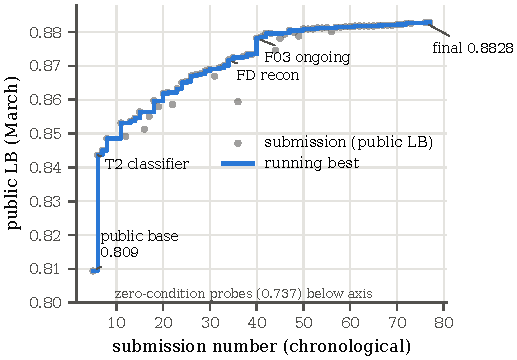
\includegraphics[width=\columnwidth]{figures/lb_progression.pdf}
\caption{Public LB of the 73 scored submissions in \file{all\_submitted\_notebooks/README.md} (from \#5; the two
zero-condition probes at 0.737 are off-axis) and the running best. Generated by \file{make\_figures.py}.}
\label{fig:lb}
\end{figure}

\begin{figure}[t]
\centering
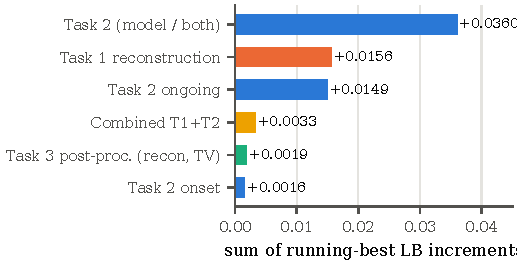
\includegraphics[width=\columnwidth]{figures/lb_by_task.pdf}
\caption{Running-best public-LB increments from 0.80939 to 0.88281, summed by the task the submission changed. Increments are
measured against the running best, not against a common base, so they are an attribution, not a clean ablation. Chain:
\file{figures/lb\_steps.csv}.}
\label{fig:bytask}
\end{figure}

Figure~\ref{fig:lb} shows the LB history and Table~\ref{tab:prog} the main steps. Our first own Task~2 model (LightGBM cell classifier with
expected-IoU decoding) lifted the public notebook~\cite{soukeaizenz} from 0.80939 to 0.84357. Two probes with one condition zeroed then
measured the LB IoU directly ($\Delta S=0.3\cdot0.5\cdot\text{IoU}$): onset 0.743 and ongoing 0.747 at 0.84855. Over the whole campaign,
Task~2 changes account for $+0.053$ of public LB (including $+0.034$ from the first classifier), Task~1 for $+0.016$, the Task~3
post-processing for $+0.002$ and one combined step for $+0.003$ (Fig.~\ref{fig:bytask}). The organizer's
persistence baseline scores 0.2518 on $S_\text{queue}$.

\begin{table}[t]
\centering
\caption{Selected steps of the public-LB progression (March; each row builds on the row above unless noted in \file{TRACKER}).}
\label{tab:prog}
\setlength{\tabcolsep}{3pt}
\begin{tabular}{@{}lllr@{}}
\toprule
Kernel & Task & Change & LB \\
\midrule
exp000 & all & public notebook~\cite{soukeaizenz} & 0.80939 \\
probe-t2 & T2 & LightGBM cell classifier + exp.-IoU decode & 0.84357 \\
final v2 & T1 & LightGBM residual, profile-free & 0.84855 \\
swap-v5 & T2 & ongoing prior-free & 0.85309 \\
swap-v9 & T2 & weekday-class priors & 0.85639 \\
combo6 & T1 & 511 leaves, $4\times$ rows & 0.86327 \\
combo9 & T1 & transductive rows & 0.86707 \\
c16 & T1 & bag of 8 FTA members & 0.87009 \\
c17 & T3 & FD-gated reconciliation & 0.87176 \\
c20 & T3 & 1-D TV & 0.87271 \\
e1 & T1 & + FD-feature bag & 0.87334 \\
e3 & T2 & selection-faithful ongoing (F03) & 0.87817 \\
e5 & T2 & onset same-scenario prior (sp4) & 0.87961 \\
g3 & T2 & all-finite inputs + occupancy & 0.88092 \\
h1 & T1 & blackout ramp member & 0.88129 \\
i4 & T1 & blackout specialist & 0.88176 \\
k1 & T1 & CatBoost member & 0.88198 \\
k5 & T1 & XGBoost member & 0.88225 \\
k7 & T1 & flow LRTC member & 0.88259 \\
\textbf{k9 / k10} & T1 & LRTC ranks + blackout LRTC & \textbf{0.88281} \\
\bottomrule
\end{tabular}
\end{table}

\begin{figure}[t]
\centering
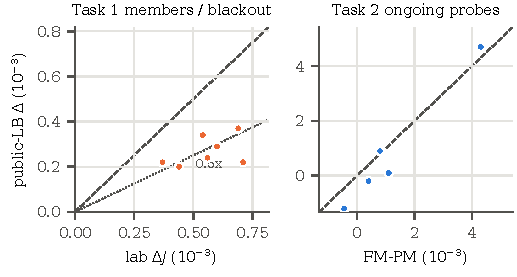
\includegraphics[width=\columnwidth]{figures/transfer.pdf}
\caption{Offline estimate versus realised public-LB delta. Left: Task~1 lab $\dJ$ of the members and blackout models that were
shipped (dashed: $y=x$; dotted: $y=0.5x$). Right: Task~2 ongoing probes, FM-PM on the validation footprint. FM-PM was calibrated on
these probes. Data with sources: \file{figdata/transfer.csv}.}
\label{fig:transfer}
\end{figure}

\textbf{Offline-to-LB transfer.} Figure~\ref{fig:transfer} (left) shows that Task~1 lab gains transferred at about 0.3--0.6$\times$. That is
expected, because the lab stand-in averages 2--4 members while production averages 17, so one extra member is diluted. The
transfer was steady enough to predict the order of magnitude of each step. For example, K9 was forecast at about $+0.0002$ and observed at
$+0.00022$. For Task~2 ongoing changes, FM-PM tracked the LB; plain OOF did not. For onset, no offline measure
predicted the LB (Sec.~\ref{sec:neg}).

\textbf{Estimated component levels.} At 0.86217 the components were estimated as $S_\text{ODME}\approx0.994$,
$S_\text{FD}\approx0.99$, $S_\text{state}\approx0.94$, $S_\text{LWR}\approx0.51$ and $S_\text{queue}\approx0.78$ (\emph{estimates}, solved from LB probes;
\file{research/SCORE\_GAP\_ANALYSIS.md}). Since then, $+0.0095$ of LB has come from Tasks~1 and 3 and $+0.0111$ from Task~2 (\file{figures/lb\_steps.csv}).

\textbf{Measured component levels of the final pick.} On 2026-11-04 three probes zeroed one block of the exact tfb-k9 file
(\file{kaggle\_jobs/probe\_k9.py}; all other rows unchanged). Zeroing the onset queue rows gave 0.76597, the ongoing rows 0.75602 and the
path flows 0.68406, against 0.88281. Because each block enters the composite linearly, the drops give public-LB onset IoU $0.779$,
ongoing IoU $0.845$, $S_\text{queue}=0.812$ and $S_\text{ODME}\approx0.994$ (zero path flows taken as $S_\text{ODME}=0$). The remaining
$0.440$ is $0.35\,S_\text{state}+0.05\,S_\text{FD}+0.10\,S_\text{LWR}$. Onset is the weakest block. In new-scenario proxies, 57--78\,\% of its loss comes from windows whose predicted cells miss the
true queue entirely (\file{analysis/TRANSFER\_ANALYSIS\_2026-10-08.md}). \textbf{Private leaderboard.} The selected pair (tfb-k9, tfb-k10) scored 0.87590 on the private (April) leaderboard, rank 83, against 0.88281 on the public (March) leaderboard. The drop of 0.0069 between the two independently generated months is in line with the per-panel window noise of Task~2 (Sec.~\ref{sec:val}) and with the organizers' warning that the two leaderboards will not agree.

\section{What did not work}\label{sec:neg}
\begin{table}[t]
\centering
\caption{Onset changes that looked good offline but lost on the public LB (\file{TRACKER}).}
\label{tab:onset}
\setlength{\tabcolsep}{3pt}
\begin{tabular}{@{}llr@{}}
\toprule
Change & Offline evidence & LB $\Delta$ \\
\midrule
30/70 main/prior-free blend & local onset worse & $-0.0039$ \\
50/50 CatBoost / LGB & pseudo-March $+0.018$ & $-0.0021$ \\
CatBoost bag + stage-2 stacker & CV $+0.0064$, 4/4 folds & $-0.0130$ \\
leave-one-day-out priors & pseudo-March $+0.018..0.028$ & $-0.0050$ \\
early-month mixture prior & forecast $+0.004$ & $-0.0014$ \\
all-finite inputs for onset & train OOF $+0.004..0.006$ & $-0.0011$ \\
\bottomrule
\end{tabular}
\end{table}

\textbf{Onset tuning.} Table~\ref{tab:onset} lists six onset changes that passed CV or pseudo-March and then lost on the LB, some
heavily. An onset window has a median of about 3 queued cells, so one flipped cell moves its IoU by 0.3--0.6. Forty windows cannot separate a
real gain from noise, and pseudo-March labels (observed cells only, masked histories) differ from the official noise-free labels.
After these results we stopped probing onset on the LB. The pre-registered April onset extensions (location columns, March
re-weighting; \file{TRACKER} EXP\_T2\_PV2) also failed their gates.

\textbf{Task 2 ongoing.} Several ideas failed. 103 extra history features (``ogfeat'') looked good offline (official-like $+0.020$) but lost
$-0.0012$ on March, because two growth calls specific to the scenario were wrong. Calibration (Platt, isotonic, power, per-step size factors)
did not help, since the decoder's size had no bias. A kinematic shock-wave gate removed correct growth cells. Reversing link order
in W/S panels gave $-0.003$. A regime switch for windows that start mid-run ($-0.0002$ LB) did not help either. Raw space-time patches, a vehicle-count / jam-length estimate, occupancy on the
April model and blending in 30\,\% persistence ($-0.0018$ LB) all failed.

\textbf{Late Task~2 tests (pre-registered, train and pseudo-March only).} (i) \emph{Simulation-augmented onset.} A cell-transmission
model driven by each train day's boundary data was meant to generate scenarios with redrawn ramp demand. It failed its realism check: the
released ramp flows barely move the mainline (slope 0.06--0.21 of $\Delta q$ on net ramp flow, a conserving model gives 1), and the
simulator placed onsets correctly in 62\,\% of windows against 98\,\% for the train location prior. Bottleneck activation in the
generator is therefore not driven by ramp demand. (ii) \emph{Half-hour phase.} Train onsets cluster at :35 and :05 (612 and 346 against
93 and 118 at :30 and :00), so demand appears to step every 30 minutes. Phase columns gave $+0.018$ IoU on 5 seeds but $+0.003$
$[-0.008, +0.014]$ on 15 fresh seeds; per-seed noise on 214 windows (about $\pm0.02$) is as large as the effect. (iii) \emph{Joint
trajectory decoding}, choosing a whole translated train trajectory by expected IoU instead of the top-$m$ cells, changed no window on
the production-like model and lost $-0.164$ IoU on a weaker one.

\textbf{Task 1 / 3.} Other approaches also failed. A Kalman/RTS smoother ($-0.019$ composite), interpolating per-lane flow instead of total
flow, a density model $q=\hat k\hat v$, per-regime models and an L1 density model all lost. A day-grid U-Net (raw speed RMSE 2.5 against 1.7 for
LightGBM), ExtraTrees, ridge and kNN-day members failed too. Density time-interpolation post-processing from public notebooks was negative in
all 27 settings (our features already contain the interpolation), and so was a conservation-aware projection, whose best variant reached only
$+0.00006$. The LWR projection failed for a structural reason: on these panels the
station-to-station flux estimate is noisier than the signal.

\textbf{Task 4.} A $\lambda$ sweep and IRLS gave no gain over the organizer's NNLS.

\section{Reproducibility}\label{sec:repro}
\textbf{Entry script.} \file{consolidation/run\_all.py} rebuilds either pick from the competition release with one command. Each
stage is the original Kaggle kernel, vendored with only its I/O lines changed (each marked \texttt{\# [TFB]}, which a static test
enforces). A template test checks that every rendered Task~1 member part equals its original source, compared as an AST.
Pick A (tfb-k9) is rebuilt with \texttt{python run\_all.py --data-root <kaggle\_public> --work-dir ./work --pick A3 --recipe full}
and pick B (tfb-k10) with \texttt{--pick B3}; \texttt{--list} prints the stage plan.
The code is submitted as \file{TrafficFlowBench\_Hack2Publish.zip}. Its root \file{README.md} lists the contents; the entry script is \file{code/run\_all.py}, and the folder called \file{consolidation/} in this report is \file{code/} in the zip.

\textbf{Compute.} All members ran on Kaggle CPU kernels (4 vCPU, about 30\,GB RAM). A Task~1 LightGBM member takes 4.6--8.8\,h over its 2--3 panel parts,
with a peak of 28.0\,GB. The CatBoost members take 15.7\,h per seed over 4 parts and the XGBoost member 4.2\,h
(\file{consolidation/lineage\_K9.json}). The previous pick (tfb-j4) was measured at 107--111 Kaggle CPU-hours in the full recipe. Adding the k
generation gives an \emph{estimated} 143--147 CPU-hours for tfb-k9. On one 8-core, 32\,GB Linux machine the earlier full recipe was
estimated at 63--68\,h of wall time. On Kaggle the consolidated light stages took: the k9 step (LRTC member, FD reconstruction, TV) 1121\,s including the parity
comparison; the Task~4 + Task~1 mix + k9 chain from the member outputs 3599\,s; each queue assembly about 110\,s.
We did not run the full recipe end to end on one machine before the deadline, so the per-stage Kaggle times above are measured and the totals are estimates. The largest measured peak is 28.0\,GB (one LightGBM member part), so a machine with at least 32\,GB of RAM is required; the stages are independent per member part and can run in parallel.

\textbf{Environment.} Python 3.13 Kaggle image (digest in \file{consolidation/ENVIRONMENT.md}). The parity runs used numpy 2.1.3, pandas 2.3.3,
scipy 1.16.3, LightGBM 4.6.0, CatBoost 1.2.10 and pyarrow 23.0.1. These versions, plus XGBoost 2.1.4, are pinned in \file{code/requirements.txt}. The original kernels did not log a \texttt{pip freeze} of their image; the parity runs on the later image reproduced them exactly or to floating-point order (Sec.~\ref{sec:repro}).

\textbf{Determinism.} Seeds, thread counts and operation order are those of the original kernels. Each stage runs in its own process with
\texttt{PYTHONHASHSEED=0} and 4 OMP/BLAS threads. CatBoost reproduced exactly across images (agreement 1.000000). Light stages (onset,
Task~1 mix, recon/TV, assembly, Task~4) matched the Kaggle outputs exactly. The original LightGBM kernels did not fix LightGBM's
histogram construction, so reruns of the Task~2 ongoing models differ in a few dozen of 87{,}000 cells. The private-score bound for this
is about 0.0012, within the organizers' 1\,\% tolerance (\file{consolidation/README.md}). The consolidated stages therefore run LightGBM with
\texttt{deterministic=True, force\_row\_wise=True}.

\textbf{Kaggle parity of the final picks (2026-11-03/04).} Seven parity kernels ran the consolidated code on Kaggle CPU images and compared
every row with the submitted files (\file{consolidation/kaggle\_parity/}). The k5d mix, the k9 step and the B3 assembly are byte-identical to
tfb-k5d, tfb-k9 and tfb-k10. The full Task~4 $\rightarrow$ Task~1 mix $\rightarrow$ k9 chain, rebuilt from the member outputs, matches
tfb-k9 exactly on all 6{,}735{,}795 state rows and 70{,}708 path flows. The A3 assembly matches tfb-k9 exactly on queue rows and path flows;
its state rows differ by at most $3.6\times10^{-15}$\,km/h and $9.1\times10^{-13}$\,veh/h (floating-point order), and its upload scored
0.88281 on the public LB, the same as tfb-k9. Task~4 alone matches the j4/j3 files exactly.

\textbf{Task~2 rerun with post-origin rows removed.} We ran the organizers' check ourselves (\file{award/t2\_postT/}). Every Task~2
producer used by the picks was rerun on release-shaped trees with all rows after a cut deleted, at cuts placed on each window's own $T$,
in three deletion styles (rows emptied, files removed, later windows removed from the index). Across about 4 million compared cells no
prediction for a window with $T\le$ cut changed. The test exposed crashes of the original code on empty inputs (an empty slot-$T$ frame, a
split without windows); the consolidated stages carry 18 guarded lines (marked \texttt{[POSTT-R1..R6]}) that leave the full-data output
byte-identical.

\section{Limitations and conclusion}
Only 40 windows per condition are scored per month, so Task~2 effects below about 0.002 cannot be seen on the LB, and our onset
model is still tuned mainly offline. The April picks hedge one structural uncertainty (scenario sharing) and cannot resolve it. Most of the
compute goes into a Task~1 ensemble whose last members add $+0.0002$ each. Our main lessons apply beyond this competition.
Reproduce the evaluation's \emph{selection} process before training on it. Physics enters this score mainly through noise in the reconstructed
density, so physics-aware post-processing should target that noise. Pre-registered gates with controls and a measured offline-to-LB transfer ratio
made a 73-submission campaign much less prone to fitting LB noise.

\section*{Acknowledgments}
We thank the TrafficFlowBench organizers for the benchmark and their forum answers. Our pipeline started from the public notebook of
S\=osuke Aizen~\cite{soukeaizenz}. The 1-D TV idea follows a public notebook by Hisernberg. The month-level low-rank completion
idea was suggested by a public notebook by plarmuseau, and the CatBoost member settings follow a public notebook by anubisyy. All code in our
final pipeline was written or re-implemented by the team, and no external data was used.

\begin{thebibliography}{9}
\bibitem{tfb} TrafficFlowBench organizers, ``TrafficFlowBench: a four-task freeway traffic benchmark for the 2026 IEEE Big Data
Cup,'' repository README and docs (\file{repo/}), and Kaggle competition ``2026 IEEE Big Data -- Traffic Flow Bench,'' 2026.
\bibitem{soukeaizenz} S. Aizen, ``[0.809 LB] Open-sourcing our physics-consistent 4-task pipeline,'' Kaggle notebook and forum
post 742980, 2026.
\bibitem{lwr1} M. J. Lighthill and G. B. Whitham, ``On kinematic waves II: a theory of traffic flow on long crowded roads,''
\emph{Proc. R. Soc. A}, vol. 229, pp. 317--345, 1955; P. I. Richards, ``Shock waves on the highway,'' \emph{Oper. Res.}, vol. 4,
pp. 42--51, 1956.
\bibitem{liu2013} J. Liu, P. Musialski, P. Wonka and J. Ye, ``Tensor completion for estimating missing values in visual data,''
\emph{IEEE TPAMI}, vol. 35, no. 1, pp. 208--220, 2013.
\bibitem{chambolle2004} A. Chambolle, ``An algorithm for total variation minimization and applications,'' \emph{J. Math. Imaging
Vis.}, vol. 20, pp. 89--97, 2004.
\bibitem{lawson} C. L. Lawson and R. J. Hanson, \emph{Solving Least Squares Problems}. Prentice-Hall, 1974.
\bibitem{lgbm} G. Ke et al., ``LightGBM: a highly efficient gradient boosting decision tree,'' in \emph{NeurIPS}, 2017.
\bibitem{catboost} L. Prokhorenkova et al., ``CatBoost: unbiased boosting with categorical features,'' in \emph{NeurIPS}, 2018.
\bibitem{xgb} T. Chen and C. Guestrin, ``XGBoost: a scalable tree boosting system,'' in \emph{KDD}, 2016.
\end{thebibliography}

\end{document}
